\documentclass[12pt]{report}

\usepackage[utf8x]{inputenc}
\usepackage[francais]{babel}
\usepackage{amsmath}
\usepackage{cancel}
\usepackage{amssymb}
\usepackage{mathrsfs}
\usepackage[pdfmenubar=true]{hyperref}
\usepackage[top=2cm, bottom=2cm, left=2cm, right=2cm]{geometry}
\usepackage{fancyhdr}
\usepackage{sectsty}
\usepackage{soul}
\usepackage{tikz}
\usetikzlibrary{intersections}
\usetikzlibrary{patterns}
\usetikzlibrary{trees}
\usepackage{wrapfig}
\usepackage{multirow}
\setlength{\fboxsep}{2mm}
\usepackage{color}
\usepackage{colortbl}
\usepackage{fancybox}

\rhead{\leftmark}
\lhead{\rightmark}
\cfoot{\thepage}

\hypersetup{%
    pdfborder = {0 0 0}
}

\chapterfont{\centering}
\renewcommand*\thesection{\arabic{section}}
\renewcommand\thechapter{\Roman{chapter}}

\makeatletter
\renewcommand{\@chapapp}{}
\makeatother

\everymath{\displaystyle}
\begin{document}
\arraycolsep=1.4pt\def\arraystretch{2.2}

\begin{titlepage}
\begin{minipage}[t]{0.4\textwidth}
	\begin{flushleft}
	\hspace{0.1cm}Projet C première année\\
	\end{flushleft}
\end{minipage}\hfill
\begin{minipage}[t]{0.4\textwidth}
	\begin{flushright}
	\textsc{Info 1}
	\textsc{Mario Like} \\
	\href{https://github.com/Gaulois94/ET3\_Project\_C/}{https://github.com/Gaulois94/ET3\_Project\_C}
	\end{flushright}
\end{minipage} ~\\[1cm]

\begin{minipage}[t]{0.5\textwidth}
	\begin{flushleft}
		\begin{tabular}{>{\bfseries}l@{:}>{\itshape}l}
		Elève 1 & Mickael Francisco SERENO\\
		Mail & \href{mailto:mickael-francisco.sereno@u-psud.fr}{mickael-francisco.sereno@u-psud.fr}\\
		\end{tabular}
	\end{flushleft}
\end{minipage}\hfill
\begin{minipage}[t]{0.4\textwidth}
	\begin{flushright}
		\begin{tabular}{>{\bfseries}l@{:}>{\itshape}l}
		Elève 2 & Stacy GROMAT\\
		Mail & \href{mailto:stacy.gromat@u-psud.fr}{stacy.gromat@u-psud.fr}\\
		\end{tabular}
	\end{flushright}
\end{minipage}\hfill

~\\[1cm]
\begin{center}
 
\includegraphics[width=7cm]{logoPolytech.jpg}~\\[1.5cm]
 \end{center}
 \hrule
	\begin{center}
	{ \huge \bfseries Projet C Mario Like de première année\\[0.4cm] }
	\hrule
	\end{center}
	\begin{center}
 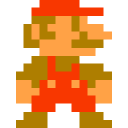
\includegraphics[width=7cm]{marioIcon.png}~\\[1.5cm]
 \end{center}
\vfill
\begin{center}
	07 Janvier 2015 - 01 Fevrier 2015
\end{center}
\end{titlepage}


\renewcommand\thepage{}
\tableofcontents
\newpage
\renewcommand\thepage{\arabic{page}}
\setcounter{page}{1}

\section{Objectifs}

\paragraph{} Les objectifs du projet furent principalement d'implémenter les concepts de bases d'un jeu Mario Bros, c'est à dire le fait de traverser une carte créée avec des blocs \footnote{Tiles dans le code} et des ennemis afin de passer au niveau suivant. En ce sens, nous avons réussi à reproduire ce concept à son stade le plus basique. En effet nous avons pu recréer les systèmes des pièces, des sols, des points de départs (qui n'est certe pas affiché mais existe dans notre format de carte) et des points d'arrivés (le château). De plus, nous avons aussi créé les ennemis les plus basiques appelés Goombas dans le code.

\paragraph{} Il était aussi prévu de faire une gestion des records, de plusieurs cartes (nous voulions en proposer deux) et même d'un mode deux joueurs.

\subsection{Objectifs réussis}

\paragraph{} Nous avons donc réussi de nombreux mécanismes dans ce projet, notamment tout ce qui tourne autour de la gestion de la carte et des intéractions avec elles. Le personnage, les ennemis ainsi que blocs / pièces fonctionnent. Des points de départ et d'arrivé ont aussi été définis.
\paragraph{} De la musique évènementielle a aussi été créée (les sauts et les pièces pour le moment, mais en rajouter est très simple). Une musique de fond a aussi été rajoutée (celle du jeu original, Nintendo Copyright).
\paragraph{} Le menu Option a aussi été créé, où nous pouvons modifier les touches du personnage, et désactiver le son. D'autres options pourront aussi y apparaître ultérieurement si besoin.

\subsection{Objectifs non réalisés}
\paragraph{} Nous n'avons ici géré qu'une seule carte. En gérer une autre est simple, mais par manque de temps, nous avons du faire des compromis. Nous n'avons pas non plus géré les records comme prévu au début. Nous avons préféré avoir un jeu fonctionnel au lieu d'avoir des choses en plus et n'avoir rien du tout de fonctionnel pour l'utilisateur. Enfin, le mode deux joueurs n'est pas présent, comme prévu initialement. Nous nous sommes rendu compte que ceci ne rapporterai pas beaucoup dans le jeu, et donc nous avons décidé de ne pas le faire (décision prise quelques jours après que le cahier des charges ait été envoyé).

\section{Difficultés / Solutions}

\subsection{Difficultés}
\paragraph{} La principale difficulté d'un jeu tel que Mario Bros est de le rendre suffisament modulable pour avoir des perspectives d'améliorations facilement implémentables. De plus, le jeu pouvant vraiment être complet, le format de carte est un choix important du projet.
\paragraph{} La SDL nous étant imposées, il fallait la comprendre et surtout l'utiliser le plus simplement possible (dans le sens que le code devait rester logique) pour avoir un projet le plus modulable.

\subsection{Solutions}
\subsubsection{Orienté Objet}

\paragraph{} Pour la modularité du projet, nous avons opté pour une approche objet du problème. Bien que le C n'est pas un langage orienté objet, nous avons pu utiliser les concepts de bases d'un code orienté objet, à savoir :
\begin{itemize}
	\item Le principe d'héritage
	\item Le principe de polymorphisme
	\item Les méthodes et attributs
\end{itemize}

\paragraph{} Pour l'héritage, nous avons tout simplement profité des caractéristiques des structures en langage C, à savoir que l'on peut caster et avoir accès aux N premiers bits d'une structure comme si celle-ci était un autre type de données.
\paragraph{} Pour le polymorphisme, les pointeurs sur fonctions étaient ce qui semblaient le plus approprié. Il suffit juste de changer ce pointeur (qui fait partie des attributs de la structure) vers la bonne méthode et tout fonctionnera.

\subsubsection{Moteur de jeu}

\paragraph{} Avec le concept d'objet utilisable, nous avons pu développer un petit mais fonctionnel moteur de jeu. Les animations, textes, sprites, Widgets sont utilisables dans l'ensemble, et ne dépendent pas du jeu lui même.
\paragraph{} Nous avons de plus utilisé le concept de Context afin d'avoir des parties du code bien définies. Un Context est tout simplement un morceau du jeu qui se suffit à lui même. Le menu Start, le menu d'Options et le jeu en lui même (InGame) sont des Contexts qui ne dépendent de personne pour subsister. Les variables qu'ils échangent sont enregistrées dans globalVar.c / globalVar.h
\paragraph{} Pour décompiler la carte, nous avons utilisé expat \footnote{\url{http://expat.sourceforge.net/}} qui est un parser évènementiel. À chaque fois qu'il rencontre une balise ouvrante (fermante), il appelera la fonction correspondante définie par XML\_SetElementHandler en donnant en paramètre une donnée qu'on aura choisi (ici ce sera notre structure Map), les attributs de la balise et son nom. Le format de la carte est donné en commentaire dans include/Map.h.
\paragraph{} Nous en avons profité pour créer un parser CSV basique. En effet, les rangées de blocs sont écrites en CSV, et il nous fallait donc écrire un parser.
\paragraph{} Chaque tile a un type écrit dans le fichier xml. La carte récupère ce type ce qui permet de créer le bon object au bon moment. Chaque object n'a donc pas un type standard, mais est propre à ce qu'il est. Leur utilisation est donc grandement simplifiée, et rajouter des objects est assez simple en soit.

\subsubsection{Les évènements}

\paragraph{} Pour les évènements, nous n'avons pas voulu qu'une seule entité gère tous les évènements. Nous donnons donc successivement les évènements aux objets qui peuvent potentiellement récupérer à la volée cet évènement et laisser cette entité gérer son évènement toute seule. Comme les évènements au clavier ne sont pas continus, nous utilisons des variables en plus pour connaître le dernier état d'un évènement (par exemple stillDown dans Player.h qui permet de savoir si la touche est toujours enfoncée)

\subsubsection{IAs}

\paragraph{} Chaque ennemi (en théorie, dans ce code il n'y en a qu'un seul) est lié à une fonction IA. En effet la difficulté d'une IA, en plus d'avoir un code complexe, est la manière d'accéder aux informations distantes (le Contexte InGame, le Player, etc.). Nous avons donc utilisé des pointeurs sur fonction qui serviront de fonction IA.

\section{Qui fait quoi ?}

\subsection{Stacy GROMAT}
\paragraph{} Stacy GROMAT aura créer tout les contexts ainsi que le fonctionnement du joueur. InGame, Start et Options sont donc ses travaux principaux. Elle a de plus coder les classes List et ResourcesManager, qui sont tout simplement des implémentations de std::list et std::map (à leur version la plus basique) disponible en C++. 

\subsection{Mickaël SERENO}
\paragraph{} L'éditeur de carte étant le sien, Mickaël SERENO aura décompiler la carte, créé les différentes classe Ennemies / Tiles et les classes Drawables / Widgets.

\subsection{Ensemble}
\paragraph{} On ne pouvait pas partir chacun de son coter sans avoir fait ensemble une base solide. Nous avons donc décider ensemble de comment le projet sera construit, comment on gèrera les évènements, comment les classes intéragissent entre elles, etc.

\subsection{Internet}
\paragraph{} Nous n'avons malheureusement pas pu créer nos propres fichiers images, fonts et sons. Tout les fichiers autres que xml présents dans le dossier Resources viennent donc de internet. Les fichiers images viennent toutes de \url{http://www.mariouniverse.com/} 

\section{Perspectives}

\subsection{À faire}

\paragraph{} Les perspectives seront tout d'abord de terminer ce qui était prévu dans le cahier des charges, à savoir une gestion des records et de plusieurs cartes.
\paragraph{} Ensuite, nous pourrions prendre en compte plusieurs blocs, comme ceux qui font des dégats, ou encore des blocs bonus. De nouveaux ennemis seront aussi appréciables.
\paragraph{} Des animations de début, de fin, une meilleur introduction seront des plus visuels conséquents pour un jeu vidéo. Revoir donc le côté artistique serait donc fort appréciable.

\subsection{Ce qui permet de le faire}

\paragraph{} Certaines techniques d'algorithmes ont été mis en place pour faciliter l'amélioration du programme. On ne reviendra pas sur le côté objet qui est la principal.
\paragraph{} On va d'abord parler des tableaux pour faire des traitements identiques. Prenons par exemple notre manière de gérer les collisions. Nous avons 4 points remarquable pour chaque personnages / ennemis qui sont les 4 coins d'un rectangle, et nous testons pas exemple chaque point pour voir s'il n'est pas en collision avec une pièce (pour notre personnage). Ce que nous avons fait c'est créé un tableau temporaire remplit avec les pointeurs sur les tiles présentent sur chacun des points du rectangle, et nous testons dans une boucle toutes les tiles du tableaux, en vérifiant si la tile est toujours disponible (l'utilité de la variable Tile$::$canDestroy)
\paragraph{} Prenons maintenant le cas des containers. Nous avons recréé la classe std$::$map présent en C++ dans sa version la plus basique qui s'appelle dans notre code ResourcesManager. On ne l'utilise qu'une seul fois pour garder en mémoire les Fonts. En absolue on n'utilise qu'une seul font dans notre projet, mais supposons que nous en voulons plusieurs. Le cas de ResourcesManager est justement la pour régler ce problème, faire en sorte que les resources soient le plus simplement possible accéssible et avoir le minimum de variables répétitives.
\paragraph{} Ces containers utilisent des pointeurs sur void$*$. En effet, dans un projet écrit en C, tout les pointeurs ont exactement la même taille en mémoire (on parle bien du pointeur et non vers ce quoi il pointe). Nous pouvons donc écrire que tout les pointeurs sont des void*, c'est à dire un pointeur brut, qui a pour caractéristique d'avoir une taille définis par le système (32 bits pour les systèmes 32 bits, et 64 bits pour les systèmes 64 bits). Pour avoir des containers génériques donc, nous avons utilisé ces void$*$ que nous castons dans notre type correct après. (ceci peut aussi être utilisé pour les int et char qui rentre dans la taille définis par un pointeur).
\paragraph{} Les techniques de callback sont aussi utilisées. En effet les pointeurs sur fonctions pour tout les objets Active servent à que plusieurs objets appellent la même fonction si besoin. Ici pour un développement assez faible il n'est pas très utile, mais plus le jeu sera poussé, plus le nombre de répétitions risquent de s'agrandir. Par exemple si plusieurs ennemies utilisent la même IA, mais sont fondamentalement différentes, les pointeurs sur fonctions IA prennent tout leur sens.
\paragraph{} La technique de Context est aussi l'une des techniques permettant par exemple de rajouter des Menus pause, une introduction animée de notre programme de manière très simple (au Context près). Par exemple pour l'introduction, il suffira de créer un context introduction, d'y faire une animation dans la fonction Context$::$run puis de retourner le prochain Context (par exemple START) une fois l'animation terminée. Chaque Context est indépendant et se comporte comme un mini programme (au données global près).

\section{Comment l'utiliser ?}

\paragraph{} Le choix de l'outil pour compiler est cmake \footnote{\url{https://cmake.org/}}. Il permet de créer un Makefile adapté à notre machine (donc utilisable sous Windows, Linux et Mac), en plus de rajouter des fonctionnalités telles que la copie de dossier comme Resources et libs si on est sous Windows. Les librairies et includes sous Windows sont fournis dans l'archive. Cependant pour linux, il vous faudra les bibliothèques suivantes :

\begin{itemize}
	\item SDL2
	\item SDL2\_image
	\item SDL2\_ttf
	\item SDL2\_mixer
	\item expat
\end{itemize}

\paragraph{} L'utilisation de cmake est défini dans le README pour linux. Sous windows, merci de lire ceci : \url{https://cmake.org/runningcmake/}. En pratique, il suffira de dire où sont les sources, où est-ce que vous voulez compiler, d'appuyer sur configure et ok. Le Makefile sera ainsi créé et vous pourrez compiler via mingw32-make par exemple.
\paragraph{} Le code source est disponible sur \url{https://github.com/Gaulois94/ET3\_Project\_C} ou en ligne de commande sous linux : git clone https://github.com/Gaulois94/ET3\_Project\_C.git
\paragraph{} Les touches du jeu sont définies dans le context Options. Vous pouvez changer les touches en cliquant sur leur valeur (par défaut c'est GAUCHE, DROIT et HAUT pour se déplacer). Start lancera le jeu et Quit (ou Alt+F4 / croix / killall / etc.) fermera le programme. Le programme aura été testé sous valgrind pour vérifier si on ne perd pas trop de mémoire (fuite mémoire) au fur et à mesure que le programme tourne (très important).


\end{document}

